\documentclass{article}
\usepackage{pgffor}
\usepackage{filecontents}
\usepackage{pdfpages }
\usepackage{graphicx} 
\usepackage{a4wide}
\usepackage{here} 
\usepackage{tabularx}
\usepackage[colorlinks]{hyperref}
\usepackage[german]{babel}
\usepackage[utf8]{inputenc}
\usepackage[T1]{fontenc}
\usepackage[3D]{movie15}
\usepackage{booktabs} 
\usepackage{eurosym}
\usepackage{verbatim}
\usepackage{amsmath}
\usepackage{textcomp}
\usepackage{caption}
\usepackage{setspace} 
\usepackage{geometry}
\usepackage{pdfpages}
\geometry{a4paper, top=25mm}

\setcounter{tocdepth}{5}  % Ebenen für Aufnahme in das Inhaltsverzeichnis
\setcounter{secnumdepth}{4}  % Ebenen für Nummerierung


\begin{document}

\begin{titlepage}

\begin{center}


% Oberer Teil der Titelseite:

\includegraphics[width=0.15\textwidth]{./Files/logo.png}\\[1cm]    

\textsc{\LARGE Zwischenbericht}\\[1.5cm]

\textsc{\Large Bremen}\\[0.5cm]


% Title
\newcommand{\HRule}{\rule{\linewidth}{0.5mm}}
\HRule \\[0.4cm]
{ \huge \bfseries Team Gamma}\\[0.4cm]

\HRule \\[1.5cm]

% Author and supervisor
\begin{minipage}{0.4\textwidth}
\begin{flushleft} \large
\emph{Autoren:}\\
Robin \textsc{Bley}\\
Alexander \textsc{Brennecke}\\
Alexander \textsc{Feldmann}\\
Marc \textsc{Huisinga}\\
Kevin \textsc{Neumeyer}\\
Till \textsc{Schlechtweg}\\
Steffen \textsc{Wißmann}
\end{flushleft}
\end{minipage}
\hfill
\begin{minipage}{0.4\textwidth}
\begin{flushright} \large
\emph{Betreuer:} \\
Harm \textsc{Hörnlein-Roboom}\\
Frank \textsc{Marschall}
\end{flushright}
\end{minipage}

\vfill

% Unterer Teil der Seite
{\large \today}

\end{center}

\end{titlepage}

\newpage
\thispagestyle{empty}
\tableofcontents
\thispagestyle{empty}
\newpage
\setcounter{page}{1}

% Import des Kurzberichtes
\section{Kurzbericht}
Insert Kurzbericht here!!!

% Import der Aufgabenliste
\section{Aufgabenliste}

\subsection{Aufgabenliste Hardware}
\begin{table}[H]
  \centering
    \begin{tabular}{p{3cm}p{7cm}p{3cm}rrr}
    \toprule
    \textbf{Aufgabe} & \textbf{Unteraufgabe} & \textbf{Status} \\
    \midrule
  	Planung & & abgeschlossen \\
	& Erstellung Verteilung der Arbeitspakete & abgeschlossen \\
	& Erstellung von PAP und PSP & abgeschlossen \\
	\midrule
	Bergungssystem & & abgeschlossen \\
	& Fallschirmdesign entwickeln & abgeschlossen\\
	& Bau der Fallschirme & abgeschlossen\\
	\midrule
	Sensorik & & in Bearbeitung\\
	& TMP006 testen und Codeentwicklung & abgeschlossen\\
	& Adafruit GPS testen und Codeentwicklung & in Bearbeitung\\
	& BMP180 testen und Codeentwicklung & abgeschlossen\\
	& Sparkfun UV testen und Codeentwicklung & in Bearbeitung\\
	& Transceiver testen und Codeentwicklung & in Bearbeitung\\
	& Geeignete Stromversorgung entwickeln & in Bearbeitung\\
	& Sharp Feinstaubtest und Codeentwicklung & abgeschlossen\\
	\midrule
	Beagleboard & & abgeschlossen\\
	& Auswahl der Programmiersprache & abgeschlossen\\
	& Aktualisieren der Software auf dem Beagle & abgeschlossen\\
	\midrule
	Dosendesign & & in Bearbeitung\\
	& Dosendeckel anfertigen & abgeschlossen\\
	& Ummantelung der Dose anfertigen & abgeschlossen\\
	& Dosendesign innerhalb der Dose & in Bearbeitung\\
	& Platzmanagement in der Dose & in Bearbeitung\\
	& Kabelmanagement in der Dose & in Bearbeitung\\
	& Stabilitätstest der Dose & ausstehend\\
	& Befestigung des Landungssystems an der Dose & ausstehend\\
	& Löten und Integration aller Komponenten & ausstehend\\
	\midrule
	Dokumentation & & in Bearbeitung\\
    \bottomrule
    \bottomrule
    \end{tabular}%
    \caption{Ausgaben}
  \label{tab:aufgabenliste_hardware}%
\end{table}%

\subsection{Aufgabenliste Software}
\begin{tabular}{p{3cm}p{7cm}p{3cm}rrr}
\hline
  \textbf{} & \textbf{Erledigt} & \textbf{in Bearbeitung} \\ \hline
  Oberfläche & Verwaltung von Satelliten implementieren & Option zum Auswählen der Location des Log-Files  \\ 
  & Menüs für die Handhabung von Features erstellen &  \\
  & Icons zum starten und stoppen von Verbindungen zwischen Clients oder Satelliten implementieren & \\ \hline
  Visualisierung & Graphvisualisierung & Autoscoroll für Visualisierungskomponenten \\
  & Kartenvisualisierung & Bugs der Kartenvisualisierung beheben \\
  & Tabellenvisualisierung & \\ \hline
  Datenimport & CSV-Dateien & \\
  & JSON-Dateien & \\ \hline
  Datenexport & KML-Format & Fehler des KML-Exports beheben \\
  & TXT-Format & \\
  & CSV-Format & \\
  & JSON-Format & \\
  & Logging der empfangenen Daten implementieren & \\ \hline
  Datenverarbeitung & USB-Schnittstelle implementieren &  \\ 
  & Input-Pipeline implementieren & \\ \hline
  Automatisierte Tests & Datenexport & Funkverbindung zum CanSat \\
  & Datenimport & \\
  & Input-Pipeline & initialisierung der Datenquellen anpassen \\
  & Netzwerkverbindung zum Smartphone & \\ \hline
  Zusammenführen der Komponenten & Oberfläche mit Exportern verbinden & Verbindung zwischen Oberfläche und CSV-Export anpassen \\ 
  & Oberfläche mit Importern verbinden & \\
  & Oberfläche mit Input-Pipeline verbinden & \\
  & Oberfläche mit Visualisierungen verbinden & \\ \hline
  Allgemeine Anpassungen & Dokumentation der Software & überarbeitung der Code-Dokumentation \\
  & Planen der Software & \\
  & Gesamte Modulstuktur überarbeiten &\\
  & interne Datentypen angepassen & \\
  & Branding erstellen & \\
  & Interfaces erstellen für Komponenten & \\
  & Ausgibige Recherche über Netbeans Plattform & \\
 \end{tabular}


% Import des detailierten Statusberichtes
\section{Detaillierter Statusbericht}
Im Nachfolgenden fassen wir in einem kurzen aber detaillierten Statusbericht den aktuellen Stand des Projektes zusammen. Der Statusbericht ist dabei in zwei kleinere Berichte aufgeteilt. Dabei handelt es sich zum einen um den Bericht der Hardware-Gruppe, welche sich mit dem Bau des Satelliten beschäftigt hat. Zum anderen handelt es sich um den der Software-Gruppe, welche sich um die Programmierung der Bodenstation und der Android-Applikation gekümmert hat. Das aktuelle Designdokument ist ebenfalls bereits sehr umfangreich, genauere Informationen über unsere abgeschlossenen und dokumentierten Arbeiten lassen sich also dort auffinden.

\subsection{Hardware-Statusbericht}
Der Schwerpunkt der Hardware-Gruppe liegt auf dem Bau und der Programmierung des Satelliten, sowie des Landesystems. Während der vergangenen Monate hat die drei-Personen-Gruppe eine Auswahl an relevanten Sensoren bestellt und diese in das System integriert. Um diese erfolgreich zu integrieren, wurden diverse Tests auf die Tauglichkeit der Sensoren durchgeführt. Eine zusätzliche Herausforderung war es, die Kompatibilität zwischen unserem Mikrocontrollerboard und den Sensoren herzustellen. Des Öfteren kam es dabei zu Komplikationen, welche uns im Endeffekt sehr viel Zeit gekostet haben.

Wir haben lange überlegt, wie wir die Sensoren innerhalb unserer Dose unterbringen, und wie wir die Dose gestalten. Da unser Mikrocontrollerboard, im Gegensatz zu dem T-Minus CanSat-Board, sehr viel Platz wegnimmt, fiel es uns lange Zeit schwer, eine geeignete Befestigung und Ausrichtung innerhalb der Dose zu finden. Schlussendlich haben wir uns für eine 3D-gedruckte Wand geeinigt. Diese teilt die Dose entlang des Durchmessers in zwei Hälften. Die eine Hälfte kann dann von dem Mikrocontrollerboard, die andere von unserer Sensorikplatine belegt werden. Sowohl das Board, als auch die Platine, können problemlos an der Wand befestigt werden.

Wir haben uns aus diversen Gründen für eine Platine entschieden. Zum einen bietet sie die Möglichkeit, die Menge an benötigten Kabeln deutlich zu verringern. Hinzu kommt, dass die Platine auch eine Befestigungsmöglichkeit für die Sensoren bietet.

Momentan ist es noch nicht möglich, die Platine innerhalb der Dose zu platzieren, da sie noch nicht die richtige Größe hat und die Sensoren noch nicht auf ihr befestigt sind. Dies wird jedoch unser nächster und auch letzter Schritt sein. Wenn die Sensorik Platine integriert ist, werden wir unsere finale Testphase einleiten, in welcher wir erst den CanSat selber und dann auch die Kommunikation mit der Bodenstation testen werden. Für diese Aufgaben existiert eine zwei Monate lange Zeitspanne zwischen August und Oktober.

Für die Kommunikation mit der Bodenstation wird aktuell noch unsere Antenne benötigt, welche noch nicht gebaut wurde. Wir haben zwar bereits konkrete Pläne für eine Helixantenne, jedoch hatten wir bis dato aus zeitlichen Gründen nicht die Möglichkeit, diese Pläne in die Realität zu übertragen.

Zusätzlich wollen wir uns in den kommenden Monaten noch weiter mit dem wissenschaftlichem Hintergrund unserer Datensammlung auseinandersetzen, da dieser bis jetzt etwas vernachlässigt wurde.

\subsection{Software-Statusbericht}
Der Schwerpunkt der Software-Gruppe liegt auf der Entwicklung der Bodenstation zum Empfangen, Verarbeiten und Visualisieren der Daten und auf der Entwicklung der Android-Applikation, welche die Aufgaben der Bodenstation als mobile Lösung erfüllen soll.

Bevor wir mit dem Schreiben der Bodenstation beginnen konnten, mussten wir uns zuerst für die Technologien entscheiden, die wir verwenden wollten. Nachdem diese Entscheidungen getroffen waren, haben wir mit der Entwicklung der verschiedenen Teilfunktionalitäten der Bodenstation begonnen und die grundlegende Architektur aufgebaut. Über die ersten Monate haben wir uns demnach hauptsächlich mit der Entwicklung der verschiedenen Features beschäftigt und uns mit den neuen Technologien, für die wir uns entschieden haben, auseinandergesetzt. Gerade mit der Technologie ``Netbeans Platform'', welche wir in der Bodenstation für eine erweiterbare Modularchitektur und eine Integration verschiedener Benutzerinterface-Komponenten genutzt haben, gab es während dem Verlauf des Projektes viele Probleme. Am Anfang bestand hauptsächlich das Problem, dass unser Versionskontrollsystemsrepository nicht mit den vielen Konfigurationsdateien klargekommen ist, welche Netbeans Platform generiert. Dies hat zu vielen Konflikten zwischen den einzelnen Versionen geführt und uns viel Zeit gekostet. Hinzu kam auch noch, dass wir während des Projektes feststellen mussten, dass uns Netbeans Platform mehr in unseren Möglichkeiten limitiert, als wir ursprünglich erwartet hatten, was selbst triviale Programmieraufgaben kompliziert werden ließ. Auch Fehler in den von uns genutzten Technologien und regelmäßige Veränderungen an der von uns geplanten Architektur haben dazu geführt, dass sich bestimmte Aufgaben in die Länge gezogen haben.

Momentan steht der Grundriss der Bodenstation. Es ist möglich, beliebige Satellitenkonfigurationen einzustellen, die Benutzeroberfläche ist größtenteils fertig und das Empfangen von Daten kann innerhalb der Bodenstation simuliert werden. Zudem ist es möglich, empfangene Daten auch anzuzeigen und beispielsweise mithilfe einer dreidimensionalen Kartenvisualisierung des Weges des Satelliten, einem Graphen oder einer Tabelle die Daten auf verschiedenste Arten zu visualisieren. Die empfangenen Daten können ebenfalls in verschiedene Formate exportiert werden, wie beispielsweise KML, welches genutzt werden kann, um den Weg des Satelliten auch auf Google Earth darzustellen.

Als nächstes werden wir uns darum kümmern, dass verschiedene Fehler, welche noch in der Bodenstation auftreten, behoben werden. Wir möchten ebenfalls den Programmcode der Applikation überarbeiten, an vielen Stellen noch verschiedene kleine Features zur Verbesserung der Nutzerfreundlichkeit hinzufügen und außerdem auch einen größeren Fokus auf die wissenschaftliche Analyse der Daten setzen, welchen momentan nur mithilfe von Visualisierungen und nicht beispielsweise mit statistischen Analysen erfolgt.

Die Android-App wurde nicht gemeinsam mit der Bodenstation und der eigentlichen Arbeit an dem Satelliten begonnen, sondern als Extra, nachdem die Arbeit an unserem Landesystem abgeschlossen war. Die Android-App soll es Nutzern im Grunde ermöglichen, Daten, welche von der Bodenstation über einen Hotspot versendet werden, in Graphen anzuzeigen. Auch hier musste man sich zuerst mit den Technologien auseinandersetzen, welche für das Erfüllen der Aufgaben nötig waren, was ebenfalls einen großen Zeitanspruch hatte. Die Entwicklung der Android-App begann auch hier nach dem Erlernen der Technologien.

Soweit ist es bei der Android-App möglich, empfangene Daten in einem statistischen Graphen und einer Empfangsdarstellung zu visualisieren, sowie den Empfang von Daten zu simulieren, damit die Applikation auch ohne eine Verbindung zum Satelliten getestet werden kann. Auch in der Android-App treten noch an verschiedenen Stellen Fehler auf, welche es nun gilt, zu beheben. Ebenfalls muss auch in der Android-App der Programmcode überarbeitet werden.

!!TODO: Was noch in der Android-App ansteht!!

\newpage

\section{Design Dokument}
Auf den folgenden Seiten ist unser Design Dokument in seiner aktuell Form zu finden. Diese Version ist auch online unter \url{https://github.com/haloshat/Apollo13_Documentation} zu finden. Dort wird das Design Dokument während des Projektverlaufes regelmäßig auf den neusten Stand gebracht.

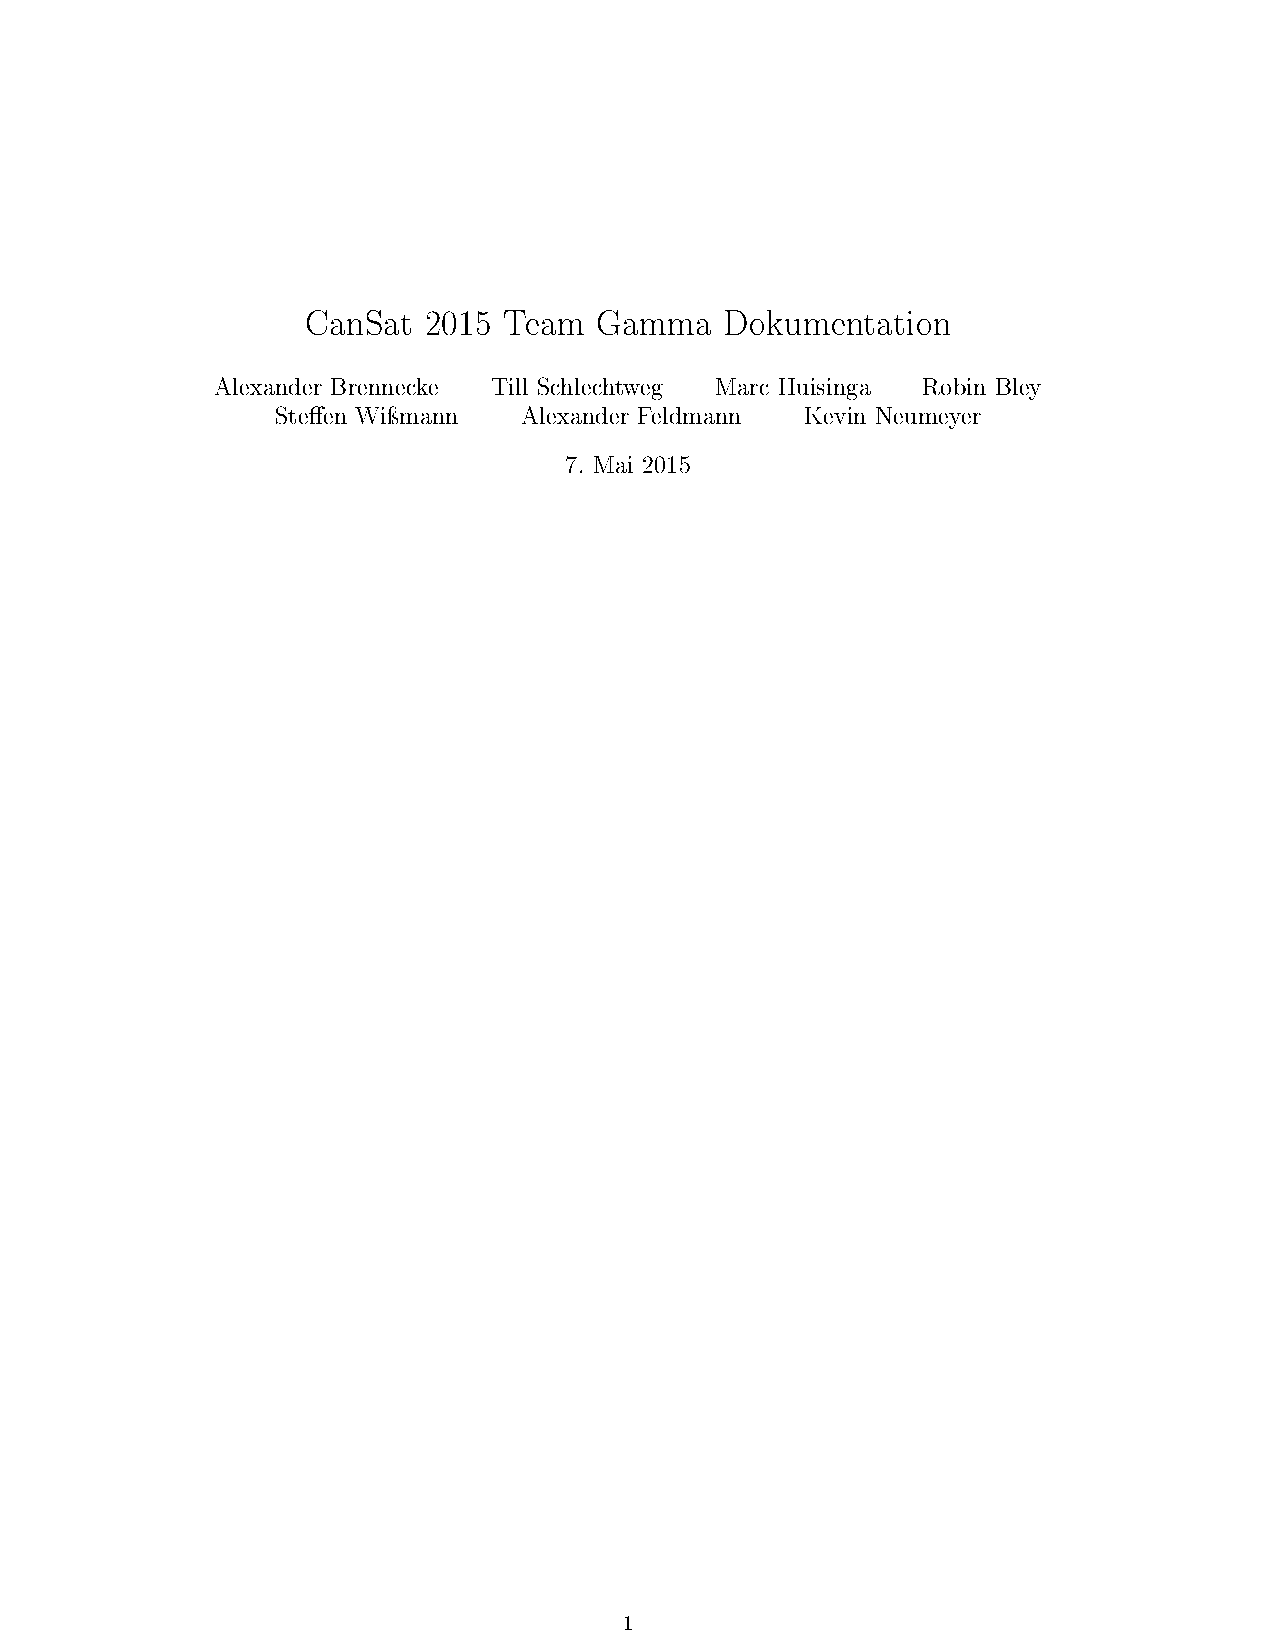
\includepdf [pages=-]{./4_Design_Document/main_doku.pdf}

\end{document}